\documentclass[12pt,a4paper,openany,oneside]{book}

\usepackage{hyperref}
\usepackage[italian]{babel}

\usepackage[utf8]{inputenc}
\usepackage[T1]{fontenc}

\usepackage{graphicx}
\usepackage[font=small,labelfont=bf,tableposition=top]{caption}

\usepackage[a4paper, top=2.2cm, bottom=2.5cm, left=2.2cm, right=2.2cm, headheight=14pt]{geometry}
            
\usepackage{listings}
\usepackage{inconsolata}
\usepackage{xcolor}
\usepackage[framemethod=tikz]{mdframed}

% Colori per il codice Python
\definecolor{commentsgreen}{rgb}{0, 0.6, 0}
\definecolor{codegray}{rgb}{0.5, 0.5, 0.5}
\definecolor{keywordpurple}{rgb}{0.77, 0.525, 0.75}
\definecolor{backcolour}{rgb}{0.12, 0.12, 0.12}
\definecolor{functionyellow}{rgb}{0.86, 0.86, 0.667}
\definecolor{basicblue}{rgb}{0.61, 0.86, 1}
\definecolor{classgreen}{rgb}{0.294, 0.745, 0.6}
\definecolor{numberyellow}{rgb}{0.686, 0.705, 0.435}
\definecolor{stringbrown}{rgb}{0.8, 0.51, 0.298}

\lstset{
    language=Python,
    basicstyle=\footnotesize\ttfamily\color{basicblue},
    numbers=left,
    numberstyle=\tiny\ttfamily\color{codegray},
    numbersep=8pt,
    tabsize=4,
    escapeinside={(*@}{@*)},
    extendedchars=true,
    breaklines=true,
    backgroundcolor=\color{backcolour},
    commentstyle=\ttfamily\color{commentsgreen},
    keywordstyle=\ttfamily\color{keywordpurple},
    stringstyle=\ttfamily\color{stringbrown},
    showspaces=false,
    showtabs=false,
    xleftmargin=17pt,
    framexleftmargin=17pt,
    framexrightmargin=5pt,
    framexbottommargin=4pt,
    showstringspaces=false,
    captionpos=b,
    morekeywords=[2]{get_teacher, get_student, get_embedding, forward, register_forward_hook, get_intermediate_features, spatial_attention_map, temporal_attention_map, compute_loss, fit_transform, interpolate},
    keywordstyle=[2]\ttfamily\color{functionyellow},
    morekeywords=[3]{TeacherModel, StudentModel, AssistantModel, AttentionTransferLoss, CombinedKDATLoss, Trainer, UCF101HFDataset, DataLoader, AdamW, TSNE, nn, torch, F, np},
    keywordstyle=[3]\ttfamily\color{classgreen},
    literate={.}{{\textcolor{white}{.}}}1 
             {=}{{\textcolor{white}{=}}}1
             {,}{{\textcolor{white}{,}}}1
             {:}{{\textcolor{white}{:}}}1
             {|}{{\textcolor{white}{|}}}1
             {+}{{\textcolor{white}{+}}}1
             {-}{{\textcolor{white}{-}}}1
             {>}{{\textcolor{white}{>}}}1
             {<}{{\textcolor{white}{<}}}1
             {*}{{\textcolor{white}{*}}}1
}

\addto\captionsitalian{
    \renewcommand{\lstlistingname}{Codice}
}

\setcounter{tocdepth}{2}
\setcounter{secnumdepth}{2}

\usepackage{amsmath}
\usepackage{amssymb}
\usepackage{float}
\usepackage{framed}
\usepackage{booktabs}
\usepackage{array}
\usepackage{subcaption}

% Pacchetti aggiuntivi per pseudo-codice
\usepackage{algorithm}
\usepackage{algpseudocode}

\emergencystretch=4em

\begin{document}

\newgeometry{top=2.5cm, bottom=3cm, left=2.5cm, right=2.5cm}
% Frontespizio
\begin{titlepage}
\centering

\vspace*{1.5cm}

{\Huge \textbf{Università degli Studi di Catania}}\\[0.5cm]
{\large Dipartimento di Matematica e Informatica}\\[2cm]

{\Large \textbf{Corso di Deep Learning: Advanced Models and Methods}}\\[0.4cm]
{\large \textbf{Relazione Progetto}}\\[2.5cm]

\rule{\textwidth}{1.2pt}\\[0.6cm]
{\Huge\bfseries Knowledge Distillation for\\[0.2cm] Mobile Action Recognition}\\[0.6cm]
\rule{\textwidth}{1.2pt}

\vspace{5.5cm}
\begin{flushright}
\begin{tabular}{@{}rl@{}}
\textbf{Autore:}          & Daniele Barbagallo\\[0.2cm]
\textbf{Matricola:}       & 1000015334\\[0.5cm]
\textbf{Docente:}         & Prof.\ Antonino Furnari\\[0.15cm]
\end{tabular}
\end{flushright}

\vspace{0.5cm}

\begin{center}
{Anno Accademico 2025/2026}
\end{center}

\end{titlepage}

\clearpage

\restoregeometry

\tableofcontents

\chapter{Introduzione}

Il riconoscimento di azioni in sequenze video rappresenta una delle sfide più rilevanti nel campo della visione artificiale. La crescente domanda di applicazioni in tempo reale su dispositivi mobili --- dalla sorveglianza intelligente alla realtà aumentata --- richiede modelli che siano al contempo accurati e computazionalmente efficienti. Tuttavia, le architetture di reti neurali 3D che raggiungono le migliori prestazioni su benchmark consolidati, come la 3D ResNet-50~\cite{he2016deep,feichtenhofer2019slowfast}, presentano decine di milioni di parametri e un costo computazionale proibitivo per il deployment su dispositivi con risorse limitate.

La \textbf{Knowledge Distillation} (KD)~\cite{hinton2015distilling} offre un paradigma elegante per affrontare questo problema: un modello ``teacher'' pesante e ad alta capacità trasferisce la propria conoscenza ad un modello ``student'' leggero, guidandone l'apprendimento tramite distribuzioni di probabilità morbide (\textit{soft targets}) piuttosto che le sole etichette rigide (\textit{hard labels}). Lo student apprende così una rappresentazione più ricca rispetto a quanto otterrebbe dal solo addestramento supervisionato, pur mantenendo un'architettura compatta adatta al deployment mobile.

\section{Obiettivi del Progetto}

Questo progetto implementa una pipeline completa di Knowledge Distillation per comprimere un modello 3D ResNet-50 (\textit{slow\_r50}), pre-addestrato su Kinetics-400~\cite{kay2017kinetics} e sottoposto a fine-tuning su UCF-101~\cite{soomro2012ucf101}, in un modello ultra-leggero MobileNet3D~\cite{sandler2018mobilenetv2}, ottenendo una riduzione dei parametri nell'ordine di 10$\times$. Gli obiettivi specifici, definiti dal Track~6 del corso, sono:

\begin{enumerate}
    \item \textbf{Teacher Model}: valutare e consolidare un 3D ResNet-50 pre-addestrato come upper bound di accuratezza.
    \item \textbf{Baseline}: addestrare un MobileNet3D da zero con sole hard labels, definendo il lower bound dell'architettura.
    \item \textbf{Knowledge Transfer}: riaddestrare lo student con le distribuzioni soft del teacher.
    \item \textbf{Valutazione}: confrontare Teacher, Baseline e Student distillato in termini di accuratezza, dimensione del modello e latenza di inferenza.
\end{enumerate}

Oltre agli obiettivi minimi, il progetto affronta tre \textit{Extra Objectives}:

\begin{itemize}
    \item \textbf{Temperature Scaling Ablation}: studio dell'effetto della temperatura $T \in \{1, 5, 10, 20\}$ sulle soft distributions del teacher.
    \item \textbf{Attention Transfer}: estensione della KD al trasferimento delle mappe di attivazione intermedie spaziali e temporali~\cite{zagoruyko2017paying}.
    \item \textbf{Visualizzazione t-SNE}: analisi qualitativa dello spazio latente per illustrare le differenze strutturali tra teacher e student~\cite{vandermaaten2008tsne}.
\end{itemize}

Inoltre, sono stati esplorati approcci avanzati non richiesti dal track, quali le \textit{Born-Again Networks}~\cite{furlanello2018born} (self-distillation iterativa MobileNet$\rightarrow$MobileNet).

\section{Organizzazione della Relazione}

La relazione è strutturata come segue. Il Capitolo~\ref{chap:background} presenta i fondamenti teorici della Knowledge Distillation e dell'Attention Transfer, con particolare attenzione all'estensione al dominio video 3D. Il Capitolo~\ref{chap:architetture} descrive le architetture dei modelli teacher e student. Il Capitolo~\ref{chap:dataset} illustra il dataset UCF-101, il protocollo sperimentale adottato e il problema del \textit{data leakage} affrontato durante lo sviluppo. Il Capitolo~\ref{chap:implementazione} dettaglia la pipeline di addestramento e le funzioni di loss implementate. Il Capitolo~\ref{chap:risultati} presenta i risultati sperimentali con analisi quantitativa e qualitativa. Infine, il Capitolo~\ref{chap:conclusioni} sintetizza i contributi e delinea i possibili sviluppi futuri.


\chapter{Background Teorico}
\label{chap:background}

Questo capitolo presenta i fondamenti teorici su cui si basa il progetto, dalla formulazione classica della Knowledge Distillation alla sua estensione con Attention Transfer per feature video 3D.

\section{Knowledge Distillation}

La Knowledge Distillation, introdotta da Hinton et al.~\cite{hinton2015distilling}, è una tecnica di compressione dei modelli in cui un modello ``teacher'' ad alta capacità guida l'addestramento di un modello ``student'' più leggero. L'intuizione fondamentale è che le \textit{soft predictions} del teacher --- ovvero le distribuzioni di probabilità ottenute applicando un parametro di temperatura $T$ ai logit --- trasportano informazioni strutturali più ricche rispetto alle sole etichette discrete. Ad esempio, un teacher che assegna una piccola probabilità alla classe ``PullUps'' quando classifica ``PushUps'' comunica allo student una relazione semantica tra queste due azioni.

\subsection{Formulazione Matematica}

Dato un input $\mathbf{x}$, il teacher produce i logit $\mathbf{z}^T$ e lo student i logit $\mathbf{z}^S$. Le distribuzioni softmax temperate sono definite come:

\begin{equation}
    \sigma_i(\mathbf{z}, T) = \frac{\exp(z_i / T)}{\sum_j \exp(z_j / T)}
\end{equation}

dove $T$ è la \textit{temperatura}. Per $T = 1$ si ottiene il softmax standard; per $T > 1$ la distribuzione diventa più uniforme, rivelando le relazioni inter-classe codificate nei logit del teacher.

La loss di Knowledge Distillation combina due componenti:

\begin{equation}
    \mathcal{L}_{\text{KD}} = \alpha \cdot T^2 \cdot D_{\text{KL}}\!\left(\sigma(\mathbf{z}^S/T) \;\|\; \sigma(\mathbf{z}^T/T)\right) + (1 - \alpha) \cdot \mathcal{L}_{\text{CE}}(\mathbf{z}^S, y)
    \label{eq:kd_loss}
\end{equation}

dove $\alpha \in [0, 1]$ bilancia il contributo della distillazione rispetto alla cross-entropy sulle hard labels $y$, e il fattore $T^2$ compensa la riduzione dei gradienti causata dalla temperatura.

\subsection{Ruolo della Temperatura}

La temperatura $T$ controlla la ``morbidezza'' delle distribuzioni di probabilità:
\begin{itemize}
    \item \textbf{$T = 1$}: le predizioni del teacher sono peaky, dominano le classi con i logit più alti; le relazioni inter-classe sono nascoste.
    \item \textbf{$T \gg 1$}: le distribuzioni si appiattiscono, rendendo visibili le correlazioni tra classi poco probabili (es. azioni simili).
    \item \textbf{$T \to \infty$}: la distribuzione converge a una uniforme, perdendo ogni informazione discriminativa.
\end{itemize}

Esiste quindi un punto ottimale che bilancia la ricchezza informativa del segnale soft con il rischio di distribuzioni troppo piatte. In questo progetto, è stato condotto uno studio ablativo sistematico con $T \in \{1, 5, 10, 20\}$ (Sezione~\ref{sec:temp_sweep}).

\section{Attention Transfer}
\label{sec:at_background}

L'Attention Transfer (AT), proposto da Zagoruyko e Komodakis~\cite{zagoruyko2017paying}, estende la KD classica al trasferimento delle \textit{feature map intermedie}. L'idea è che la distribuzione spaziale delle attivazioni --- ovvero ``dove'' la rete presta attenzione --- trasporti informazioni discriminative complementari rispetto ai soli logit finali.

\subsection{AT per Immagini 2D}

Per la classificazione di immagini, dato un tensore di feature $F \in \mathbb{R}^{B \times C \times H \times W}$, la mappa di attenzione spaziale è definita come:

\begin{equation}
    A(F) = \text{normalize}\left(\sum_{c=1}^{C} |F_c|^2\right) \in \mathbb{R}^{B \times H \times W}
\end{equation}

La loss di AT è la somma pesata degli errori MSE tra le mappe di attenzione di teacher e student su $L$ coppie di livelli:

\begin{equation}
    \mathcal{L}_{\text{AT}} = \beta \sum_{i=1}^{L} \text{MSE}\!\left(A(F^T_i),\, A(F^S_i)\right)
\end{equation}

\subsection{Estensione al Video 3D: Attenzione Spaziale e Temporale}
\label{sec:at_3d}

Nel dominio video, le feature intermedie sono tensori a 5 dimensioni: $F \in \mathbb{R}^{B \times C \times T \times H \times W}$, dove $T$ è la dimensione temporale. Un'estensione diretta dell'AT 2D al 3D --- sommare sui canali e appiattire tutte le dimensioni rimanenti --- è teoricamente scorretta perché mescola informazioni spaziali e temporali semanticamente diverse.

La soluzione adottata in questo progetto decompone l'attenzione in due componenti:

\textbf{Mappa di Attenzione Spaziale} (``dove guardare''):
\begin{equation}
    A_{\text{spaziale}}(F) = \text{L2\_norm}\left(\text{mean}_{c,t}(F^2)\right) \in \mathbb{R}^{B \times H \cdot W}
\end{equation}

Calcola la media su canali e tempo, producendo una heatmap spaziale che riassume \textit{dove} la rete presta attenzione per l'intera clip.

\textbf{Mappa di Attenzione Temporale} (``quando attivare''):
\begin{equation}
    A_{\text{temporale}}(F) = \text{L2\_norm}\left(\text{mean}_{c,h,w}(F^2)\right) \in \mathbb{R}^{B \times T}
\end{equation}

Calcola la media su canali e dimensioni spaziali, producendo un profilo temporale che riassume \textit{quando} si raggiungono i picchi di attivazione.

La loss AT combinata è:
\begin{equation}
    \mathcal{L}_{\text{AT}} = \beta_s \sum_i \text{MSE}(A^T_{s,i}, A^S_{s,i}) + \beta_t \sum_i \text{MSE}(A^T_{t,i}, A^S_{t,i})
\end{equation}

dove $\beta_s$ e $\beta_t$ sono coefficienti indipendenti per le componenti spaziale e temporale.

\subsection{Loss Totale di Distillation con AT}

La funzione obiettivo complessiva combina KD e AT:
\begin{equation}
    \mathcal{L}_{\text{totale}} = \underbrace{\alpha T^2 D_{\text{KL}} + (1-\alpha)\mathcal{L}_{\text{CE}}}_{\text{Knowledge Distillation}} + \underbrace{\beta_s \sum_i \text{MSE}(A^T_{s,i}, A^S_{s,i})}_{\text{AT Spaziale}} + \underbrace{\beta_t \sum_i \text{MSE}(A^T_{t,i}, A^S_{t,i})}_{\text{AT Temporale}}
    \label{eq:total_loss}
\end{equation}

\section{Born-Again Networks}

Le Born-Again Networks~\cite{furlanello2018born} estendono la KD alla self-distillation iterativa: uno student addestrato diventa il teacher della generazione successiva, con l'obiettivo di raffinare progressivamente le rappresentazioni interne pur mantenendo la stessa architettura. In uno scenario MobileNet$\rightarrow$MobileNet, i tensori intermedi tra teacher e student hanno la stessa dimensionalità, eliminando la necessità di interpolazione nelle mappe di attenzione. Tuttavia, come verrà discusso nella Sezione~\ref{sec:born_again}, questo approccio è soggetto a \textit{collasso generazionale} se gli iperparametri non sono calibrati per la minore confidenza del teacher non-oracolo.

\section{Visualizzazione t-SNE}

La t-SNE (t-distributed Stochastic Neighbor Embedding)~\cite{vandermaaten2008tsne} è una tecnica di riduzione dimensionale non lineare che preserva la struttura locale dei dati ad alta dimensionalità. In questo progetto viene utilizzata per proiettare gli embedding pre-classificatore dei modelli teacher, baseline e student distillato in uno spazio bidimensionale, permettendo di visualizzare il grado di separazione inter-classe e la coesione intra-classe appresa da ciascun modello.


\chapter{Architetture dei Modelli}
\label{chap:architetture}

Questo capitolo descrive le architetture dei modelli utilizzati nel progetto: il teacher 3D ResNet-50, lo student MobileNet3D e il meccanismo di accoppiamento dei layer per l'Attention Transfer.

\begin{figure}[H]
    \centering
    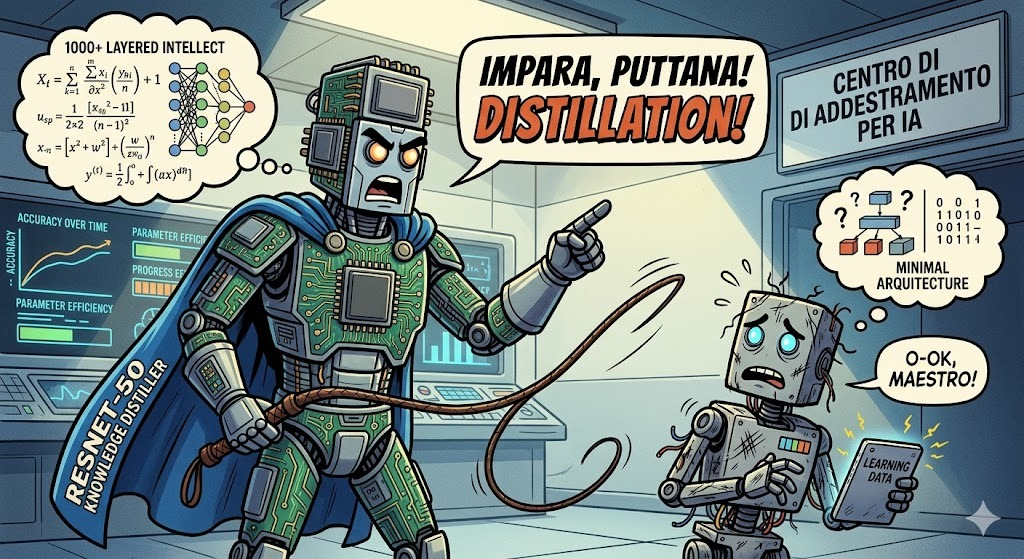
\includegraphics[width=0.7\textwidth]{parts/cap3_architetture/distil.jpeg}
    \caption{Schema concettuale della Knowledge Distillation: il modello teacher pesante trasferisce la propria conoscenza allo student leggero attraverso soft targets e, opzionalmente, mappe di attenzione intermedie.}
    \label{fig:kd_schema}
\end{figure}

\section{Teacher: 3D ResNet-50 (\texttt{slow\_r50})}

Il modello teacher è la variante \texttt{slow\_r50} di PyTorchVideo~\cite{feichtenhofer2019slowfast}, un 3D ResNet-50~\cite{he2016deep} pre-addestrato su Kinetics-400~\cite{kay2017kinetics}. L'architettura è composta da 6 blocchi sequenziali (indici 0--5):

\begin{table}[H]
\centering
\caption{Struttura del Teacher (slow\_r50). Il blocco 5 è la testa di classificazione, non uno stage di estrazione feature.}
\label{tab:teacher_blocks}
\begin{tabular}{cccc}
\toprule
\textbf{Blocco} & \textbf{Tipo} & \textbf{Output Shape} & \textbf{Descrizione} \\
\midrule
0 & ResStage & $[B, 64, T, 56, 56]$ & Conv iniziale + pool \\
1 & ResStage & $[B, 64, T, 56, 56]$ & Primo stage residuale \\
2 & ResStage & $[B, 256, T, 28, 28]$ & Secondo stage residuale \\
3 & ResStage & $[B, 512, T, 14, 14]$ & Terzo stage residuale \\
4 & ResStage & $[B, 1024, T, 7, 7]$ & Quarto stage residuale \\
5 & ResNetBasicHead & $[B, 101]$ & Global avg pool $\rightarrow$ proj \\
\bottomrule
\end{tabular}
\end{table}

La testa di classificazione originale (pre-addestrata su 400 classi Kinetics) viene sostituita con un layer lineare a 101 uscite per UCF-101. Il pooling spaziale-temporale viene reso adattivo (\texttt{AdaptiveAvgPool3d(1,1,1)}) per supportare qualsiasi dimensione di input. Il fine-tuning utilizza SGD con learning rate 0.0007, weight decay $10^{-3}$, batch size 12 e scheduler cosine annealing per 50 epoche.

\section{Student: MobileNet3D}

Lo student è un'architettura MobileNetV2~\cite{sandler2018mobilenetv2} adattata alle convoluzioni 3D per l'elaborazione video. L'architettura si basa su blocchi \textit{Inverted Residual} 3D con convoluzioni depthwise separabili:

\begin{enumerate}
    \item \textbf{Pointwise Expansion}: convoluzione $1\times1\times1$ che espande i canali di un fattore $t$ (expansion ratio).
    \item \textbf{Depthwise 3D Convolution}: convoluzione $3\times3\times3$ con \texttt{groups=hidden\_dim}, che processa ciascun canale indipendentemente. Lo stride temporale è sempre 1, preservando la dimensione $T$.
    \item \textbf{Pointwise Projection}: convoluzione $1\times1\times1$ che proietta al numero di canali di output, senza attivazione (\textit{linear bottleneck}).
\end{enumerate}

\begin{table}[H]
\centering
\caption{Stage del MobileNet3D con le risoluzioni spaziali di output.}
\label{tab:student_stages}
\begin{tabular}{cccccc}
\toprule
\textbf{Stage} & \textbf{$t$} & \textbf{$c$} & \textbf{$n$} & \textbf{$s$} & \textbf{Output Shape} \\
\midrule
0 & 1  & 16  & 1 & 1 & $[B, 16, T, 56, 56]$ \\
1 & 6  & 24  & 2 & 2 & $[B, 24, T, 28, 28]$ \\
\textbf{2} & \textbf{6}  & \textbf{32}  & \textbf{3} & \textbf{2} & $[B, 32, T, 14, 14]$ \\
3 & 6  & 64  & 4 & 2 & $[B, 64, T, 7, 7]$ \\
\textbf{4} & \textbf{6}  & \textbf{96}  & \textbf{3} & \textbf{1} & $[B, 96, T, 7, 7]$ \\
5 & 6  & 160 & 3 & 2 & $[B, 160, T, 4, 4]$ \\
\textbf{6} & \textbf{6}  & \textbf{320} & \textbf{1} & \textbf{1} & $[B, 320, T, 4, 4]$ \\
\bottomrule
\end{tabular}
\end{table}

dove $t$ è l'expansion ratio, $c$ i canali di output, $n$ il numero di blocchi e $s$ lo stride spaziale. Gli stage evidenziati in grassetto sono quelli utilizzati per l'Attention Transfer.

Il classificatore è composto da una convoluzione finale $1\times1\times1$ a 1280 canali, adaptive average pooling 3D, dropout (0.2) e un layer lineare a 101 classi. Il training del baseline utilizza AdamW~\cite{loshchilov2019adamw} con learning rate 0.0005, weight decay 0.01 e cosine annealing per 60 epoche.

\section{Confronto Dimensionale}

\begin{table}[H]
\centering
\caption{Confronto tra Teacher e Student in termini di parametri, dimensione e latenza di inferenza.}
\label{tab:model_comparison}
\begin{tabular}{lccc}
\toprule
\textbf{Modello} & \textbf{Parametri} & \textbf{Dimensione (MB)} & \textbf{Latenza (ms)} \\
\midrule
3D ResNet-50 (Teacher) & $\sim$33.4M & $\sim$128 & -- \\
MobileNet3D (Student)  & $\sim$2.5M  & $\sim$9.5 & $\sim$1.8 \\
\bottomrule
\end{tabular}
\end{table}

Il rapporto di compressione è superiore a \textbf{13$\times$} in termini di parametri e \textbf{13$\times$} in dimensione del modello, rispettando ampiamente il target di 5--10$\times$ richiesto dal track.

\section{Accoppiamento dei Layer per l'Attention Transfer}
\label{sec:layer_pairing}

L'accoppiamento corretto tra i layer del teacher e quelli dello student è cruciale per un efficace Attention Transfer. La scelta è guidata dalla similitudine semantica e dalla compatibilità delle risoluzioni spaziali:

\begin{table}[H]
\centering
\caption{Accoppiamento delle feature map per l'Attention Transfer.}
\label{tab:feature_pairing}
\begin{tabular}{ccccc}
\toprule
\textbf{Coppia} & \textbf{Teacher} & \textbf{Shape Teacher} & \textbf{Student} & \textbf{Shape Student} \\
\midrule
1 & Blocco 2 & $[B, 256, T, 28, 28]$ & Stage 2 & $[B, 32, T, 14, 14]$ \\
2 & Blocco 3 & $[B, 512, T, 14, 14]$ & Stage 4 & $[B, 96, T, 7, 7]$  \\
3 & Blocco 4 & $[B, 1024, T, 7, 7]$ & Stage 6 & $[B, 320, T, 4, 4]$ \\
\bottomrule
\end{tabular}
\end{table}

Si noti che la dimensione temporale $T$ è identica tra teacher e student a tutti i livelli, poiché entrambi i modelli utilizzano stride temporale pari a 1. Questo permette un trasferimento diretto dell'attenzione temporale senza interpolazione. Le differenze nelle risoluzioni spaziali (es. $28\times28$ vs $14\times14$) vengono gestite tramite interpolazione bilineare 2D, come descritto nella Sezione~\ref{sec:at_bug}.


\chapter{Dataset e Protocollo Sperimentale}
\label{chap:dataset}

\section{UCF-101}

Il dataset UCF-101~\cite{soomro2012ucf101} è un benchmark consolidato per il riconoscimento di azioni, composto da 13\,320 video suddivisi in 101 classi di azioni umane (sport, attività quotidiane, interazioni con oggetti). I video sono estratti da clip di YouTube e presentano sfide realistiche: variabilità di illuminazione, sfondi complessi, occlusioni parziali e variazioni intra-classe significative.

\subsection{Caricamento e Pre-processing}

Il progetto utilizza il backend \texttt{flwrlabs/ucf101} di Hugging Face, che fornisce i frame pre-estratti dei video. Il data loading pipeline opera come segue:

\begin{enumerate}
    \item \textbf{Campionamento temporale}: per ciascun video vengono campionati $N = 24$ frame tramite campionamento segmentato uniforme. Durante il training, viene applicato un jitter temporale casuale all'interno di ciascun segmento.
    \item \textbf{Trasformazioni spaziali}: i frame vengono ridimensionati a 128 pixel sul lato corto, seguiti da random crop a $112\times112$ (training) o center crop (evaluation). Si applica random horizontal flip con probabilità 0.5.
    \item \textbf{Normalizzazione}: ogni frame viene normalizzato secondo la media e deviazione standard di Kinetics ($\mu = 0.45$, $\sigma = 0.225$ per tutti i canali).
    \item \textbf{Formato}: il tensore risultante ha shape $[C, T, H, W] = [3, 24, 112, 112]$, coerente con le convenzioni PyTorchVideo.
\end{enumerate}

\section{Il Problema del Data Leakage}
\label{sec:data_leakage}

Una sfida critica affrontata durante lo sviluppo è stata l'identificazione e la correzione di un \textit{data leakage} tra training e validation set. UCF-101 organizza i video per \textit{gruppi}: video della stessa classe possono provenire dalla stessa clip sorgente, generando clip fortemente correlate.

\subsection{Evoluzione degli Split}

Il protocollo di split è passato attraverso tre fasi:

\begin{enumerate}
    \item \textbf{Train-Test split} (fase iniziale): la validation durante il training veniva effettuata direttamente sul test set ufficiale. Questo porta a \textit{selection bias}: il checkpoint selezionato è quello che massimizza le prestazioni sul test, rendendo le metriche troppo ottimistiche.
    
    \item \textbf{Train-Eval-Test split senza group-aware} (prima correzione): viene creato un validation split interno dal training set, ma la separazione avviene per singolo campione, senza vincolare i gruppi video. Di conseguenza, clip della stessa sequenza sorgente possono trovarsi sia in train che in eval, producendo metriche artificialmente alte.
    
    \item \textbf{Train-Eval-Test split group-aware} (soluzione corretta): lo split interno viene effettuato a livello di \textbf{gruppo video}. Un'espressione regolare estrae l'identificatore di gruppo (\texttt{\_g\textbackslash d+\_}) dal video ID, garantendo che tutte le clip dello stesso video sorgente finiscano nello stesso set (train o eval). Questo elimina il leakage e produce metriche affidabili.
\end{enumerate}

\subsection{Impatto Sulle Metriche}

La differenza tra i protocolli è significativa. Con lo split non-group-aware, le accuratezze di validation raggiungevano valori sistematicamente più alti, mascherando il reale gap di generalizzazione. Con lo split group-aware, il gap tra training accuracy ($\sim$98\%) e validation accuracy ($\sim$60--65\%) diventa evidente, riflettendo la reale difficoltà del task.

\textbf{Tutti i risultati presentati nel Capitolo~\ref{chap:risultati} utilizzano esclusivamente lo split group-aware.}

\subsection{Implementazione dello Split Group-Aware}

Lo split stratificato group-aware è implementato nella funzione \texttt{\_stratified\_group\_split\_indices}. Per ciascuna classe:
\begin{enumerate}
    \item Si identificano i gruppi video unici appartenenti alla classe.
    \item I gruppi vengono mescolati con un seme fisso ($\texttt{seed} = 42$).
    \item Si assegnano interi gruppi al set di eval fino a raggiungere la \texttt{eval\_ratio} target ($20\%$), con il vincolo che almeno un campione rimanga nel train.
    \item Tutti i campioni dei gruppi non selezionati finiscono nel train.
\end{enumerate}

\section{Protocollo Sperimentale Finale}

\begin{table}[H]
\centering
\caption{Protocollo sperimentale adottato per tutti gli esperimenti safe.}
\label{tab:protocol}
\begin{tabular}{ll}
\toprule
\textbf{Parametro} & \textbf{Valore} \\
\midrule
Dataset & UCF-101 (HuggingFace backend) \\
Frame per clip & 24 \\
Crop size & $112 \times 112$ \\
Split & Group-aware stratificato \\
Eval ratio & 0.2 \\
Split seed & 42 \\
Test set & Ufficiale UCF-101 \\
\bottomrule
\end{tabular}
\end{table}

\section{Infrastruttura Computazionale}

Tutti gli esperimenti sono stati eseguiti sul cluster GPU del DMI dell'Università di Catania, gestito tramite SLURM. Le risorse principali comprendono GPU NVIDIA K80, V100 e L40S. Il progetto ha utilizzato script bash automatizzati per il lancio sequenziale di pipeline multi-stage (training $\rightarrow$ evaluation $\rightarrow$ t-SNE), con gestione dei checkpoint e fallback per la ripresa dei job interrotti.


\chapter{Implementazione della Pipeline}
\label{chap:implementazione}

Questo capitolo dettaglia le componenti chiave della pipeline di addestramento, con focus sulle funzioni di loss, la logica di training e il bug critico nell'Attention Transfer.

\section{Architettura della Pipeline}

La pipeline supporta quattro modalità operative, gestite dal parametro \texttt{mode} nella configurazione YAML:

\begin{itemize}
    \item \texttt{teacher\_finetune}: fine-tuning del ResNet-50 pre-addestrato su UCF-101.
    \item \texttt{baseline}: addestramento del MobileNet3D da zero con sola cross-entropy.
    \item \texttt{distillation}: KD logit-based con soft targets del teacher.
    \item \texttt{distillation\_at}: KD + Attention Transfer spaziale/temporale.
\end{itemize}

Tutte le modalità condividono la stessa architettura di training: ottimizzatore AdamW~\cite{loshchilov2019adamw}, scheduler cosine annealing, mixed precision con AMP (Automatic Mixed Precision), e gradient clipping a norma 1.0.

\section{Funzione di Loss Combinata}

La loss per la modalità \texttt{distillation\_at} combina tre componenti come descritto dall'Equazione~\ref{eq:total_loss}. Lo pseudo-codice seguente illustra il calcolo:

\begin{algorithm}[H]
\caption{Calcolo della loss combinata KD + AT}\label{alg:loss}
\begin{algorithmic}[1]
\Require Logit student $z^S$, logit teacher $z^T$, label $y$
\Require Feature teacher $\{F^T_i\}_{i=1}^{L}$, feature student $\{F^S_i\}_{i=1}^{L}$
\Require Temperatura $T$, $\alpha$, $\beta_s$, $\beta_t$
\State $p^S \gets \text{softmax}(z^S / T)$, $p^T \gets \text{softmax}(z^T / T)$
\State $\mathcal{L}_{\text{KD}} \gets \alpha \cdot T^2 \cdot D_{\text{KL}}(p^S \| p^T) + (1 - \alpha) \cdot \text{CE}(z^S, y)$
\State $\mathcal{L}_{\text{AT}} \gets 0$
\For{$i = 1$ \textbf{to} $L$}
    \State $A^T_s \gets \text{L2\_norm}(\text{mean}_{c,t}((F^T_i)^2))$ \Comment{Mappa spaziale teacher}
    \State $A^S_s \gets \text{L2\_norm}(\text{mean}_{c,t}((F^S_i)^2))$ \Comment{Mappa spaziale student}
    \State $A^S_s \gets \text{interp2d}(A^S_s, \text{size}=A^T_s.\text{shape})$ \Comment{Allineamento risoluzione}
    \State $\mathcal{L}_{\text{AT}} \gets \mathcal{L}_{\text{AT}} + \beta_s \cdot \text{MSE}(A^T_s, A^S_s)$
    \State $A^T_t \gets \text{L2\_norm}(\text{mean}_{c,h,w}((F^T_i)^2))$ \Comment{Profilo temporale teacher}
    \State $A^S_t \gets \text{L2\_norm}(\text{mean}_{c,h,w}((F^S_i)^2))$ \Comment{Profilo temporale student}
    \State $\mathcal{L}_{\text{AT}} \gets \mathcal{L}_{\text{AT}} + \beta_t \cdot \text{MSE}(A^T_t, A^S_t)$
\EndFor
\State \Return $\mathcal{L}_{\text{KD}} + \mathcal{L}_{\text{AT}}$
\end{algorithmic}
\end{algorithm}

\section{Il Bug del Block 5 (``Key~5'')}
\label{sec:at_bug}

Un bug critico ha impattato significativamente le prime iterazioni dell'Attention Transfer. In una versione iniziale del codice, i \texttt{FEATURE\_BLOCKS} del teacher erano configurati come $[2, 3, 4, 5]$, dove il blocco 5 corrisponde alla \textbf{testa di classificazione} (\texttt{ResNetBasicHead}), non ad uno stage residuale. Questo blocco restituisce un tensore mono-dimensionale (\texttt{[B, 101]}) dopo il pooling e la proiezione lineare.

Le conseguenze di questo errore erano molteplici:
\begin{itemize}
    \item Il tensore del blocco 5, non essendo una feature map volumetrica, produceva mappe di attenzione costanti (tutti i valori a 1.0 dopo la normalizzazione).
    \item La loss AT su questa coppia era identicamente zero, rendendo il segnale AT di fatto nullo.
    \item L'errore era \textbf{silenzioso}: nessuna eccezione, nessun warning, ma una convergenza dell'AT identica al training senza AT.
\end{itemize}

La correzione ha rimosso il blocco 5 dall'elenco, settando \texttt{FEATURE\_BLOCKS = [2, 3, 4]}.

\section{Gestione dell'Interpolazione Spaziale}

Poiché le risoluzioni spaziali di teacher e student differiscono (Tabella~\ref{tab:feature_pairing}), la mappa di attenzione spaziale dello student viene ridimensionata per corrispondere a quella del teacher. L'interpolazione avviene in 2D (non 3D), coerentemente con il fatto che le mappe spaziali hanno già aggregato la dimensione temporale:

\begin{enumerate}
    \item Si fa il reshape della mappa $A^S \in \mathbb{R}^{B \times H_S W_S}$ a $[B, 1, H_S, W_S]$.
    \item Si applica \texttt{F.interpolate} con mode \texttt{bilinear} e \texttt{align\_corners=False}.
    \item Si riduce nuovamente alla dimensione della mappa teacher $[B, H_T \cdot W_T]$.
\end{enumerate}

Per la dimensione temporale, non è necessaria alcuna interpolazione poiché $T$ è identica tra teacher e student a tutti i livelli.

\section{Warmup per la Knowledge Distillation}

È stato identificato che le prime epoche di addestramento con KD beneficiano significativamente di una fase di ``warmup'' in cui la loss KD viene esclusa e lo student viene addestrato con sola cross-entropy. Questo permette ai parametri del modello di raggiungere una regione ragionevole dello spazio dei pesi prima di essere esposti al segnale di distillazione, evitando instabilità numeriche e convergenza prematura in minimi locali sfavorevoli. Nel progetto, un warmup di 10 epoche è stato adottato come default per tutti gli esperimenti di distillazione.

\section{Mixed Precision Training}

La pipeline utilizza AMP (\textit{Automatic Mixed Precision}) per accelerare il training e ridurre l'occupazione di memoria GPU. Un problema specifico riscontrato è stato l'overflow in FP16 durante il calcolo delle mappe di attenzione: l'operazione $F^2$ su feature map con valori grandi genera overflow nel range di float16. La soluzione adottata è il casting esplicito a \texttt{float32} prima dell'operazione di potenza:

\begin{verbatim}
# Cast esplicito per stabilità numerica con AMP
f = f.float()  # float32
return (f * f).mean(dim=...)
\end{verbatim}

Questo garantisce stabilità numerica senza disabilitare AMP per l'intero training.


\chapter{Risultati Sperimentali}
\label{chap:risultati}

Questo capitolo presenta i risultati ottenuti con lo split group-aware su UCF-101. Tutti i valori di accuratezza riportati come ``Test'' si riferiscono al test set ufficiale; quelli come ``Val'' si riferiscono alla porzione di validation estratta dal training set con split group-aware.

\section{Modelli di Riferimento}

\begin{table}[H]
\centering
\caption{Performance dei modelli di riferimento sul test set ufficiale.}
\label{tab:baselines}
\begin{tabular}{lcccc}
\toprule
\textbf{Modello} & \textbf{Val Top-1} & \textbf{Test Top-1} & \textbf{Test Top-5} & \textbf{Size (MB)} \\
\midrule
Teacher (3D ResNet-50) & 92.36\% & 88.82\% & 98.18\% & $\sim$128 \\
Baseline (MobileNet3D)  & 59.18\% & 59.48\% & 82.77\% & $\sim$9.5 \\
\bottomrule
\end{tabular}
\end{table}

Il \textbf{gap} tra teacher e baseline è di circa \textbf{29.3 punti percentuali} in Top-1, confermando l'esistenza di un significativo \textit{capacity gap} tra le due architetture. Questo gap è la motivazione fondamentale per la Knowledge Distillation: trasferire allo student parte della conoscenza strutturale del teacher che non emerge dal solo addestramento con hard labels.

\section{Knowledge Distillation: Risultato Principale}

L'esperimento principale di KD utilizza temperatura $T = 8$ e $\alpha = 0.7$:

\begin{table}[H]
\centering
\caption{Confronto Baseline vs Knowledge Distillation ($T=8$, $\alpha=0.7$).}
\label{tab:kd_main}
\begin{tabular}{lcccc}
\toprule
\textbf{Modello} & \textbf{Val Top-1} & \textbf{Test Top-1} & \textbf{Test Top-5} & \textbf{$\Delta$ vs Baseline} \\
\midrule
Baseline            & 59.18\% & 59.48\% & 82.77\% & --- \\
KD ($T=8$)          & 64.57\% & 64.31\% & 87.68\% & \textbf{+4.83\%} \\
\bottomrule
\end{tabular}
\end{table}

La Knowledge Distillation produce un miglioramento significativo di \textbf{+4.83 punti percentuali} in Test Top-1 e +4.91\% in Top-5, senza alcuna modifica all'architettura del modello. Lo student distillato raggiunge il 64.31\% mantenendo la stessa dimensione di 9.5~MB e la latenza di $\sim$1.8~ms.

\begin{figure}[H]
    \centering
    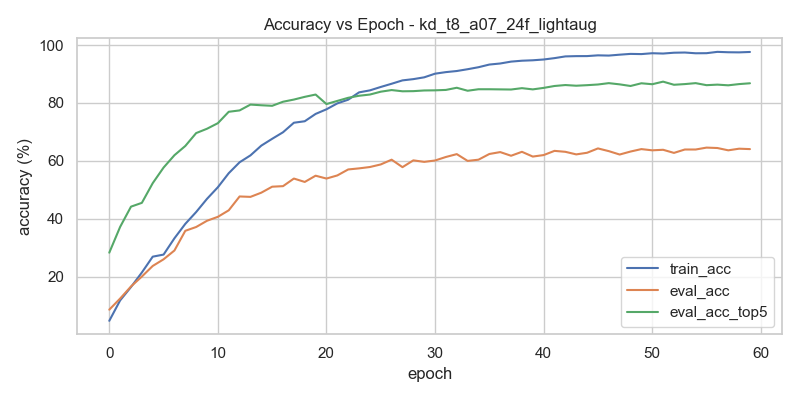
\includegraphics[width=0.8\textwidth]{parts/cap6_risultati/training_curves/kd_t8_a07_24f_lightaug_accuracy.png}
    \caption{Curve di accuracy per il training di KD con $T=8$, $\alpha=0.7$. Si noti il gap tipico tra training accuracy ($\sim$98\%) e validation accuracy ($\sim$64\%), indicativo della difficoltà del task con split group-aware.}
    \label{fig:kd_accuracy}
\end{figure}

\begin{figure}[H]
    \centering
    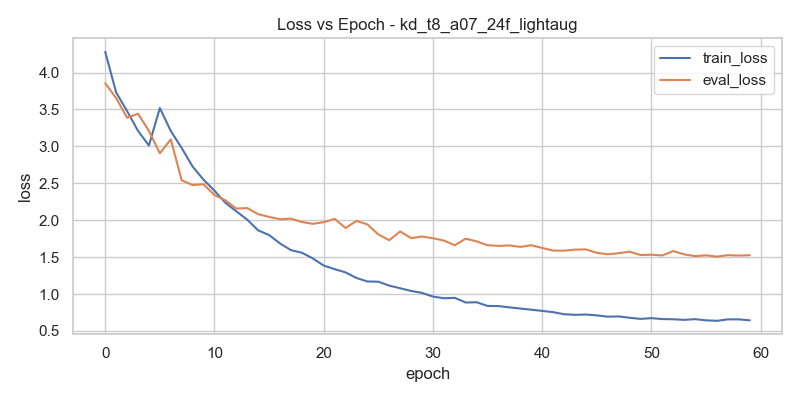
\includegraphics[width=0.8\textwidth]{parts/cap6_risultati/training_curves/kd_t8_a07_24f_lightaug_loss.png}
    \caption{Andamento della loss durante il training di KD ($T=8$).}
    \label{fig:kd_loss}
\end{figure}

\section{Temperature Scaling Ablation}
\label{sec:temp_sweep}

È stato condotto uno studio ablativo sistematico dell'effetto della temperatura sulle soft distributions del teacher:

\begin{table}[H]
\centering
\caption{Ablazione sulla temperatura con $\alpha = 0.7$ fisso.}
\label{tab:temp_ablation}
\begin{tabular}{ccccccc}
\toprule
\textbf{$T$} & \textbf{Best Val} & \textbf{Best Epoch} & \textbf{Train Acc} & \textbf{Test Top-1} & \textbf{Test Top-5} & \textbf{$\Delta$ vs BL} \\
\midrule
1  & 62.75\% & 60 & 98.44\% & 62.91\% & 85.59\% & +3.43\% \\
5  & 63.12\% & 57 & 95.87\% & 62.07\% & 87.02\% & +2.59\% \\
8  & 64.57\% & 56 & 97.59\% & 64.31\% & 87.68\% & +4.83\% \\
10 & 64.85\% & 60 & 98.28\% & 64.47\% & 87.44\% & +4.99\% \\
20 & 65.18\% & 59 & 99.05\% & \textbf{65.85\%} & \textbf{87.81\%} & \textbf{+6.37\%} \\
\bottomrule
\end{tabular}
\end{table}

\subsection{Analisi dei Risultati}

L'andamento mostra un chiaro trend crescente con la temperatura. La configurazione con $T = 20$ raggiunge la migliore Test Top-1 accuracy (\textbf{65.85\%}), con un miglioramento di \textbf{+6.37 punti percentuali} rispetto al baseline.

Questo risultato suggerisce che, per il gap di capacità significativo tra 3D ResNet-50 e MobileNet3D, temperature più alte che producono distribuzioni più uniformi risultano più efficaci. Con temperature basse ($T = 1$), le predizioni del teacher sono troppo ``peaky'' e lo student fatica a replicare la distribuzione inter-classe. Temperature alte ($T = 20$) ``smussano'' la distribuzione del teacher, esponendo relazioni tra classi che uno student limitato può meglio approssimare.

\begin{figure}[H]
    \centering
    
\includegraphics[width=0.9\textwidth]{parts/cap6_risultati/delta_accuracy_kd_vs_baseline.png}
    \caption{Delta di accuratezza (test) rispetto al baseline per ciascuna temperatura. Trend crescente con la temperatura, con picco a $T = 20$.}
    \label{fig:delta_temp}
\end{figure}

\section{Attention Transfer}
\label{sec:at_results}

L'Attention Transfer estende la KD con il trasferimento delle mappe di attenzione intermedie. Sono state testate due configurazioni:

\begin{table}[H]
\centering
\caption{Risultati dell'Attention Transfer (split group-aware). Le colonne $\beta_s$ e $\beta_t$ indicano i pesi delle componenti spaziale e temporale.}
\label{tab:at_results}
\begin{tabular}{lccccc}
\toprule
\textbf{Config} & $\beta_s$ & $\beta_t$ & \textbf{Val Top-1} & \textbf{Train Acc} \\
\midrule
KD ($T=8$, no AT)   & 0     & 0     & 64.57\% & 97.59\% \\
AT Simmetrico       & 0.05  & 0.05  & 58.25\% & 96.27\% \\
AT Temporal-Only    & 0     & 0.10  & 59.04\% & 95.87\% \\
\bottomrule
\end{tabular}
\end{table}

\subsection{Analisi del Risultato Negativo}

L'Attention Transfer non ha migliorato le prestazioni rispetto alla sola KD. Anzi, entrambe le configurazioni producono una \textbf{regressione} di 5--6 punti percentuali. Diverse ipotesi spiegano questo risultato:

\begin{enumerate}
    \item \textbf{Capacity gap spaziale}: il teacher utilizza convoluzioni standard 3D con $C \gg 1$ canali che interagiscono liberamente, producendo mappe di attenzione spaziale ricche e dettagliate. Il MobileNet3D utilizza convoluzioni depthwise separabili, dove ciascun canale è processato indipendentemente; questo limita intrinsecamente la capacità dello student di riprodurre le mappe spaziali del teacher.
    
    \item \textbf{Regularizzazione eccessiva}: il segnale AT spaziale può agire come un vincolo troppo restrittivo sulle feature intermedie, impedendo allo student di trovare soluzioni alternative compensatorie adatte alla sua architettura più limitata.
    
    \item \textbf{Dominanza del componente temporale}: l'AT puramente temporale ($\beta_s = 0$, $\beta_t = 0.1$) performa leggermente meglio del simmetrico, suggerendo che il componente spaziale è il principale responsabile della regressione.
\end{enumerate}

Questo risultato è coerente con la letteratura: il paper originale di Zagoruyko e Komodakis~\cite{zagoruyko2017paying} lavora con architetture della stessa famiglia (ResNet teacher $\rightarrow$ ResNet student), dove la similarità strutturale rende le mappe di attenzione più trasferibili.

\section{Born-Again Networks}
\label{sec:born_again}

Le Born-Again Networks tentano di migliorare lo student tramite self-distillation iterativa. Il migliore KD student ($T = 8$, $\alpha = 0.7$) diventa il teacher della Generazione~1, che a sua volta diventa teacher della Generazione~2, e così via.

\begin{table}[H]
\centering
\caption{Risultati Born-Again Networks (3 generazioni successive). Si noti il collasso progressivo delle prestazioni.}
\label{tab:born_again}
\begin{tabular}{lcccc}
\toprule
\textbf{Generazione} & \textbf{Teacher} & \textbf{Val Top-1} & \textbf{Test Top-1} & \textbf{$\Delta$ vs Gen0} \\
\midrule
Gen 0 (KD $T=8$) & ResNet-50 & 64.57\% & 64.31\% & --- \\
Gen 1              & Gen 0     & 60.78\% & 60.98\% & $-3.33$\% \\
Gen 2              & Gen 1     & 61.20\% & 60.43\% & $-3.88$\% \\
Gen 3              & Gen 2     & 59.98\% & 59.21\% & $-5.10$\% \\
\bottomrule
\end{tabular}
\end{table}

\subsection{Collasso Generazionale}

Il risultato mostra un chiaro \textbf{collasso generazionale}: ogni iterazione successiva produce prestazioni inferiori, anziché il miglioramento atteso dalla teoria~\cite{furlanello2018born}. Il collasso è progressivo: Gen~3 scende sotto il livello del baseline originale (59.21\% vs 59.48\%).

Le cause identificate:

\begin{enumerate}
    \item \textbf{Temperature non calibrata}: la temperatura $T = 2.5$ usata per la self-distillation era stata scelta per un teacher oracolo (ResNet-50 a $\sim$89\%). Un MobileNet3D a $\sim$64\% produce distribuzioni soft meno informative, e una temperatura troppo alta le rende ancora più piatte, diluendo il segnale utile.
    
    \item \textbf{Assenza di oracolo}: le Born-Again Networks presuppongono che il teacher della generazione $k$ sia almeno competente quanto quello della generazione $k-1$. Quando il teacher iniziale è già un modello limitato, il degrado della qualità del segnale si accumula.
    
    \item \textbf{Overfitting sugli artefatti}: il teacher non-oracolo commette errori sistematici che vengono amplificati e rinforzati nelle generazioni successive.
\end{enumerate}

\section{Visualizzazione t-SNE dello Spazio Latente}

La t-SNE è stata applicata alle embedding pre-classificatore per analizzare qualitativamente le rappresentazioni apprese. Per ciascuna visualizzazione, vengono selezionate 10 classi casuali e proiettate in 2D.

\begin{figure}[H]
    \centering
    
\includegraphics[width=\textwidth]{parts/cap6_risultati/tsne/tsne_comparison_4495.png}
    \caption{t-SNE a tre colonne: Teacher (ResNet-50), Baseline (MobileNet3D), e Student distillato (KD $T=8$). Il teacher mostra cluster compatti e ben separati; il baseline presenta sovrapposizione; lo student distillato mostra una struttura intermedia migliorata.}
    \label{fig:tsne_main}
\end{figure}

\begin{figure}[H]
    \centering
    
\includegraphics[width=\textwidth]{parts/cap6_risultati/tsne/tsne_teacher_baseline_at_comparison.png}
    \caption{t-SNE per i modelli con Attention Transfer: il pattern di clustering è simile a quello del baseline, confermando che l'AT non ha prodotto miglioramenti strutturali nelle rappresentazioni.}
    \label{fig:tsne_at}
\end{figure}

\begin{figure}[H]
    \centering
    
\includegraphics[width=\textwidth]{parts/cap6_risultati/tsne/tsne_born_again_final.png}
    \caption{t-SNE delle Born-Again Networks: la struttura non migliora nelle generazioni successive, coerentemente con il collasso osservato nelle metriche quantitative.}
    \label{fig:tsne_born}
\end{figure}

\section{Confusion Matrix}

Le confusion matrix normalizzate evidenziano le classi più confuse. Per leggibilità, vengono mostrate le Top-25 classi più problematiche.

\begin{figure}[H]
    \centering
    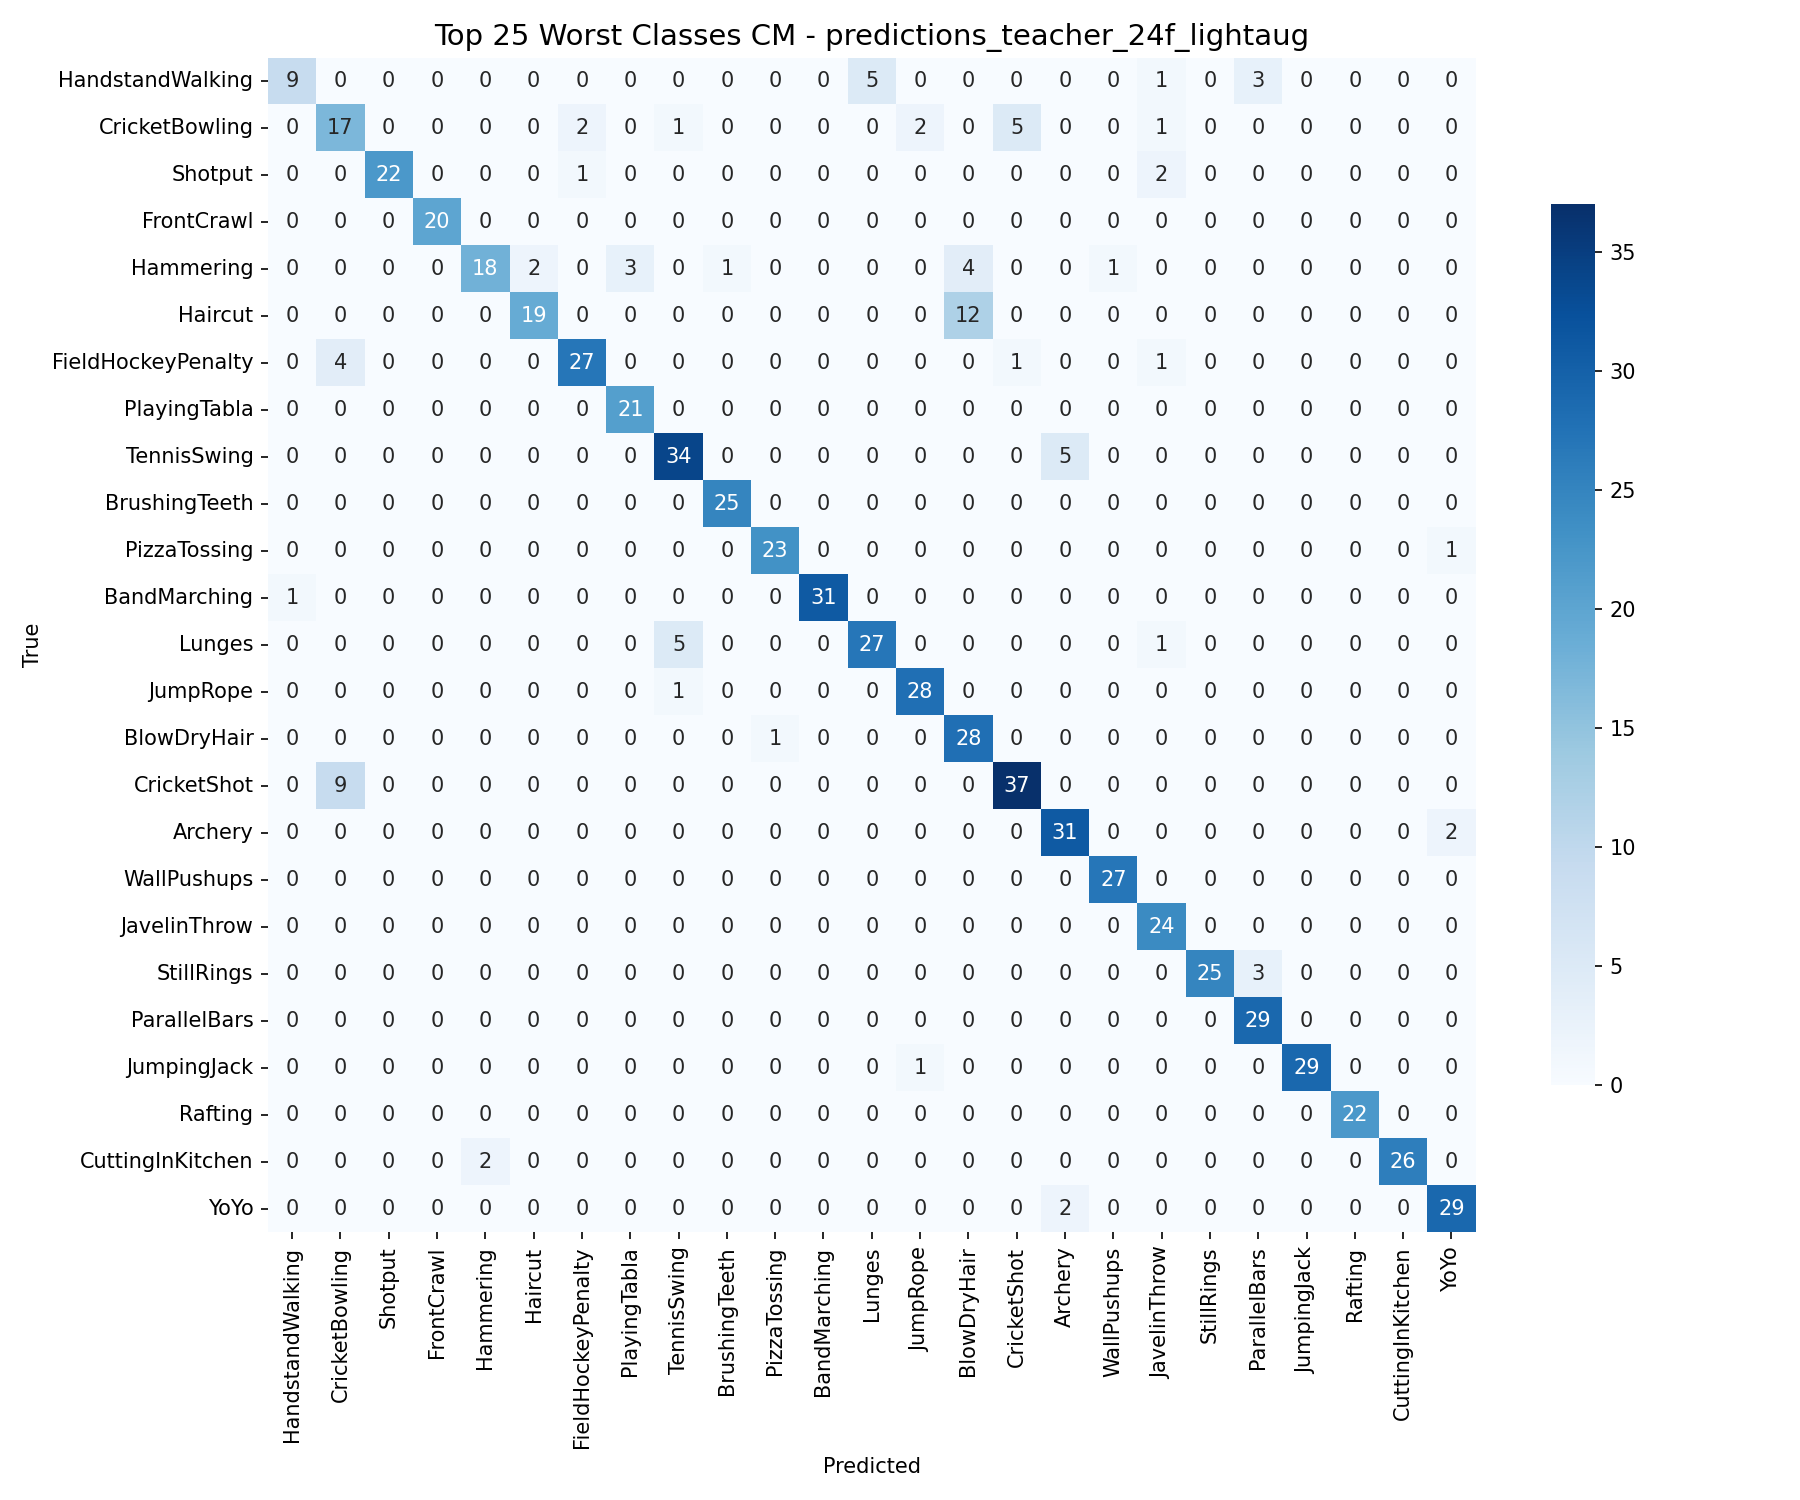
\includegraphics[width=0.85\textwidth]{parts/cap6_risultati/confusion_matrices/predictions_teacher_24f_lightaug_top25.png}
    \caption{Confusion matrix Top-25 del Teacher: errori concentrati su classi semanticamente ambigue.}
    \label{fig:cm_teacher}
\end{figure}

\begin{figure}[H]
    \centering
    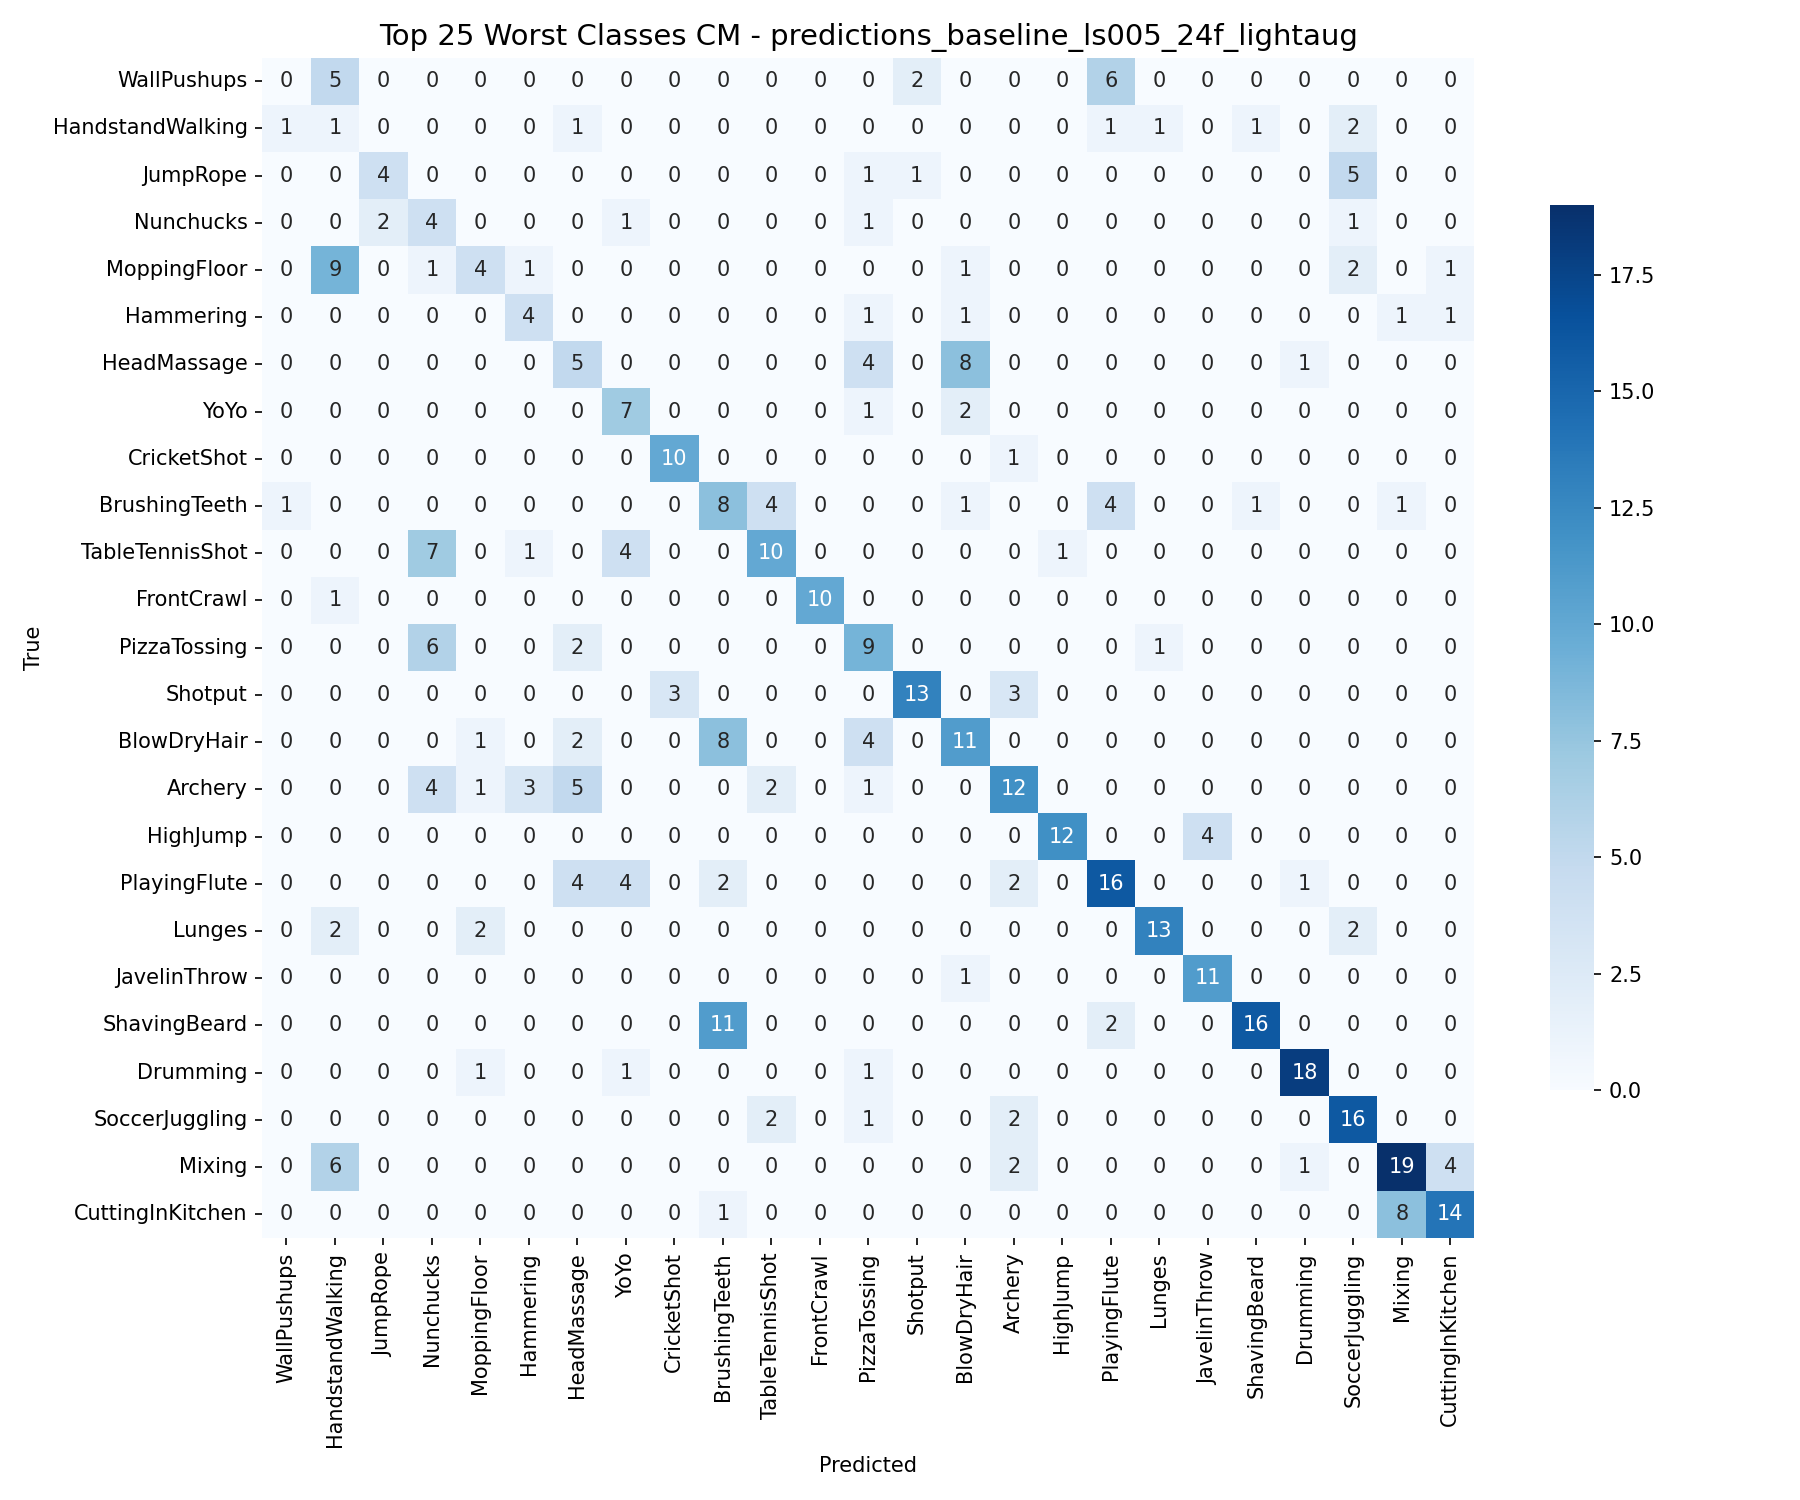
\includegraphics[width=0.85\textwidth]{parts/cap6_risultati/confusion_matrices/predictions_baseline_ls005_24f_lightaug_top25.png}
    \caption{Confusion matrix Top-25 del Baseline: pattern di confusione più diffusi, in particolare tra azioni sportive visivamente simili.}
    \label{fig:cm_baseline}
\end{figure}

\begin{figure}[H]
    \centering
    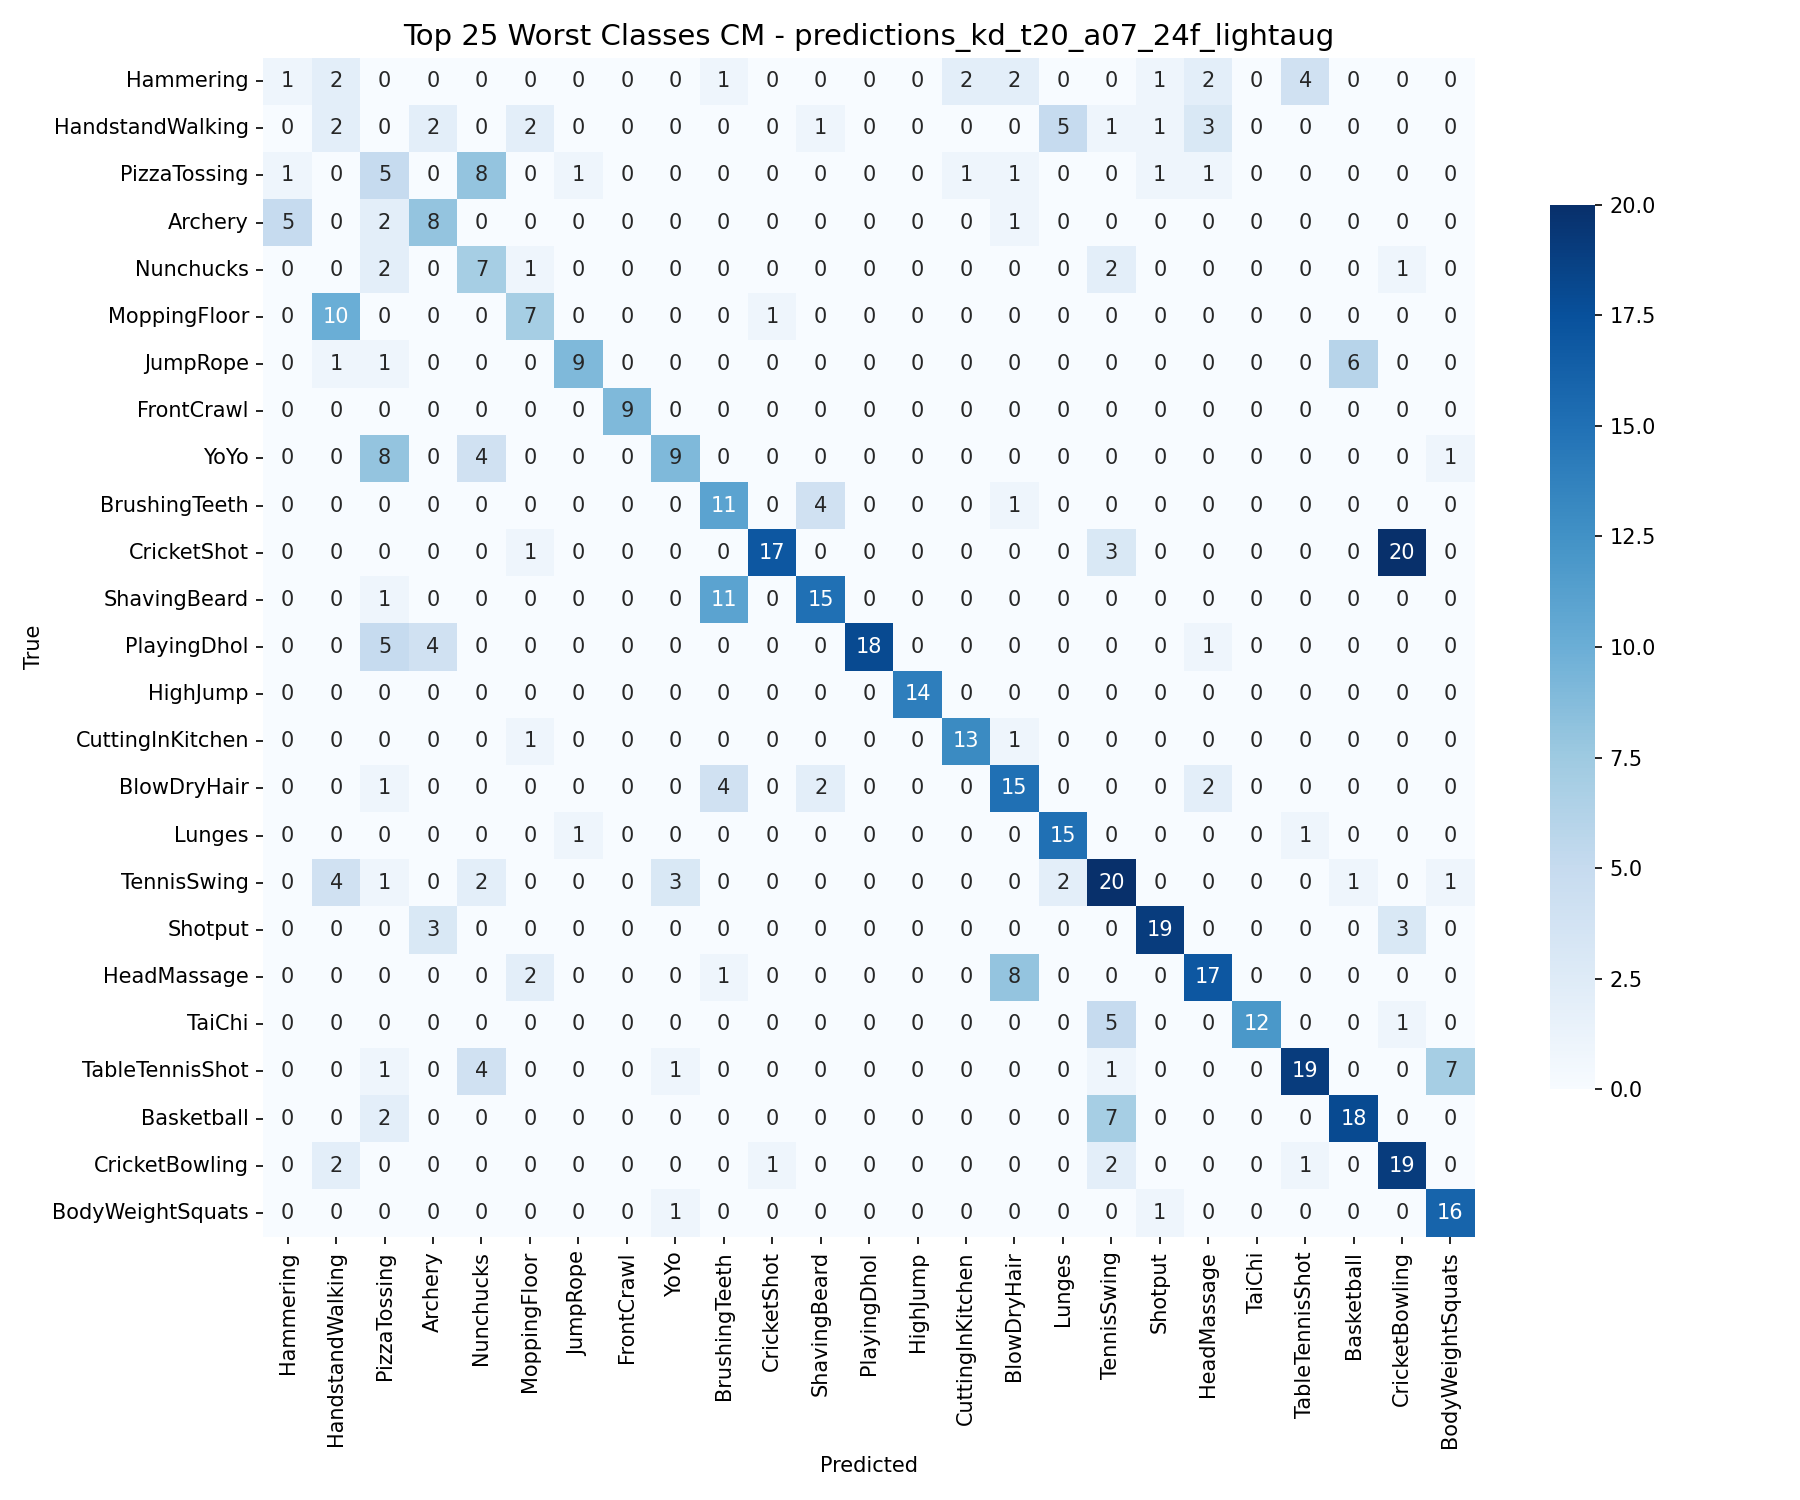
\includegraphics[width=0.85\textwidth]{parts/cap6_risultati/confusion_matrices/predictions_kd_t20_a07_24f_lightaug_top25.png}
    \caption{Confusion matrix Top-25 del migliore Student distillato (KD $T=20$): pattern di errore ridotto rispetto al baseline, evidenziando un trasferimento effettivo della conoscenza discriminativa del teacher.}
    \label{fig:cm_kd_best}
\end{figure}

\section{Riepilogo Quantitativo}

\begin{table}[H]
\centering
\caption{Riepilogo completo di tutti gli esperimenti con split group-aware.}
\label{tab:summary}
\begin{tabular}{lcccc}
\toprule
\textbf{Esperimento} & \textbf{Val Top-1} & \textbf{Test Top-1} & \textbf{Test Top-5} & \textbf{$\Delta$} \\
\midrule
Teacher (ResNet-50)     & 92.36\% & 88.82\% & 98.18\% & upper bound \\
Baseline (MobileNet3D)  & 59.18\% & 59.48\% & 82.77\% & reference \\
\midrule
KD $T=1$, $\alpha=0.7$  & 62.75\% & 62.91\% & 85.59\% & +3.43\% \\
KD $T=5$, $\alpha=0.7$  & 63.12\% & 62.07\% & 87.02\% & +2.59\% \\
KD $T=8$, $\alpha=0.7$  & 64.57\% & 64.31\% & 87.68\% & +4.83\% \\
KD $T=10$, $\alpha=0.7$ & 64.85\% & 64.47\% & 87.44\% & +4.99\% \\
KD $T=20$, $\alpha=0.7$ & 65.18\% & \textbf{65.85\%} & \textbf{87.81\%} & \textbf{+6.37\%} \\
\midrule
AT Simmetrico            & 58.25\% & --- & --- & $-5.93$\% val \\
AT Temporal-Only         & 59.04\% & --- & --- & $-5.14$\% val \\
\midrule
Born-Again Gen 1         & 60.78\% & 60.98\% & --- & $-3.33$\% \\
Born-Again Gen 2         & 61.20\% & 60.43\% & --- & $-3.88$\% \\
Born-Again Gen 3         & 59.98\% & 59.21\% & --- & $-5.10$\% \\
\bottomrule
\end{tabular}
\end{table}


\chapter{Conclusioni e Lavori Futuri}
\label{chap:conclusioni}

\section{Sintesi dei Risultati}

Questo progetto ha implementato e valutato una pipeline completa di Knowledge Distillation per la compressione di un modello 3D ResNet-50 (33.4M parametri) in un MobileNet3D (2.5M parametri) per il riconoscimento di azioni su UCF-101. I risultati principali sono:

\begin{enumerate}
    \item \textbf{KD Logit-based}: la Knowledge Distillation produce un miglioramento consistente rispetto al baseline. La configurazione migliore ($T=20$, $\alpha=0.7$) raggiunge il \textbf{65.85\%} di Test Top-1 accuracy, con un guadagno di \textbf{+6.37 punti percentuali} rispetto al baseline (59.48\%), colmando circa il \textbf{22\%} del gap tra student e teacher.
    
    \item \textbf{Temperature Scaling}: lo studio ablativo rivela un trend crescente con la temperatura nel range $[1, 20]$, suggerendo che per coppie teacher-student con capacity gap significativo, temperature alte che ``smussano'' le distribuzioni del teacher facilitano il trasferimento della conoscenza.
    
    \item \textbf{Attention Transfer}: l'estensione con AT spaziale e temporale non ha prodotto miglioramenti, anzi una regressione di 5--6 punti. Questo risultato evidenzia i limiti del trasferimento delle mappe di attenzione tra architetture strutturalmente eterogenee (convoluzioni standard vs depthwise separabili).
    
    \item \textbf{Born-Again Networks}: la self-distillation iterativa MobileNet$\rightarrow$MobileNet produce un collasso generazionale, scendendo sotto il baseline alla terza generazione. Il risultato è attribuibile alla temperatura non calibrata e all'assenza di un teacher oracolo.
    
    \item \textbf{Compressione}: il modello finale mantiene una dimensione di \textbf{9.5 MB} (vs $\sim$128 MB del teacher), una latenza di \textbf{$\sim$1.8 ms}, e un rapporto di compressione superiore a \textbf{13$\times$}.
\end{enumerate}

\section{Lezioni Apprese}

Il percorso di sviluppo ha evidenziato alcune lezioni significative:

\begin{itemize}
    \item \textbf{Data leakage silenzioso}: il leakage tra train e validation dovuto ai gruppi video di UCF-101 è un problema insidioso che produce metriche artificialmente alte senza generare errori espliciti. Lo split group-aware è essenziale per qualsiasi valutazione affidabile su questo dataset.
    
    \item \textbf{Bug silenti nelle pipeline complesse}: il bug del Block 5 nell'Attention Transfer --- che produceva mappe costanti senza alcun warning --- dimostra l'importanza della validazione delle feature intermedie tramite ispezione manuale, non solo della loss finale.
    
    \item \textbf{Stabilità numerica con AMP}: il mixed precision training richiede attenzione esplicita quando si calcolano potenze di feature map, poiché l'overflow in float16 può propagarsi silenziosamente come NaN.
    
    \item \textbf{Warmup per KD}: le prime epoche di distillazione beneficiano di una fase di warmup con sola cross-entropy, permettendo ai pesi dello student di raggiungere una regione ragionevole prima di essere esposti al segnale soft del teacher.
\end{itemize}

\section{Limiti del Lavoro}

\begin{itemize}
    \item L'ablazione sulla temperatura è stata condotta con $\alpha = 0.7$ fisso; un'analisi congiunta $T \times \alpha$ potrebbe rivelare configurazioni ottimali diverse.
    \item L'AT è stato testato con un solo set di $(\beta_s, \beta_t)$; uno sweep più ampio e un'esplorazione di tecniche di accoppiamento alternative (FitNets~\cite{romero2015fitnets}, proiezione lineare) potrebbero produrre risultati diversi.
    \item Le Born-Again Networks sono state testate con temperatura fissa; un decay della temperatura attraverso le generazioni potrebbe mitigare il collasso.
    \item Il progetto utilizza un singolo split seed; la riproducibilità dei risultati andrebbe verificata su split multipli.
\end{itemize}

\section{Lavori Futuri}

\begin{enumerate}
    \item \textbf{Progressive distillation}: utilizzare temperature decrescenti nelle Born-Again Networks per mantenere la qualità del segnale attraverso le generazioni.
    \item \textbf{Feature projection AT}: inserire layer lineari trainabili tra le feature del teacher e dello student per ridurre il mismatch architetturale nell'AT.
    \item \textbf{Distillazione multi-teacher}: combinare i segnali di teacher con architetture diverse per produrre soft targets più robusti.
    \item \textbf{Deployment reale}: integrare il modello compresso in un'applicazione mobile con benchmark di latenza su dispositivi edge (Raspberry Pi, smartphone Android).
    \item \textbf{Dataset più complessi}: estendere la valutazione a Kinetics-400 o HMDB-51 per verificare la generalizzabilità dei risultati.
\end{enumerate}

\section{Dichiarazione sull'Uso dell'IA}

Coerentemente con la policy del corso, si dichiara che durante lo sviluppo del progetto sono stati utilizzati strumenti di intelligenza artificiale generativa (GitHub Copilot, Claude) come supporto per: la scrittura di codice boilerplate, il debugging di errori, la consultazione della documentazione di PyTorch e PyTorchVideo, e l'automazione della pipeline di testing. Le decisioni architetturali, la strategia sperimentale e l'interpretazione dei risultati sono state interamente formulate dall'autore.


\bibliographystyle{plain}
\bibliography{references}

\end{document}
